\documentclass{article}
\usepackage[utf8]{inputenc}
\usepackage{polski}


\usepackage{lmodern,microtype}

\usepackage[simplified]{pgf-umlcd}
\begin{document}
	
	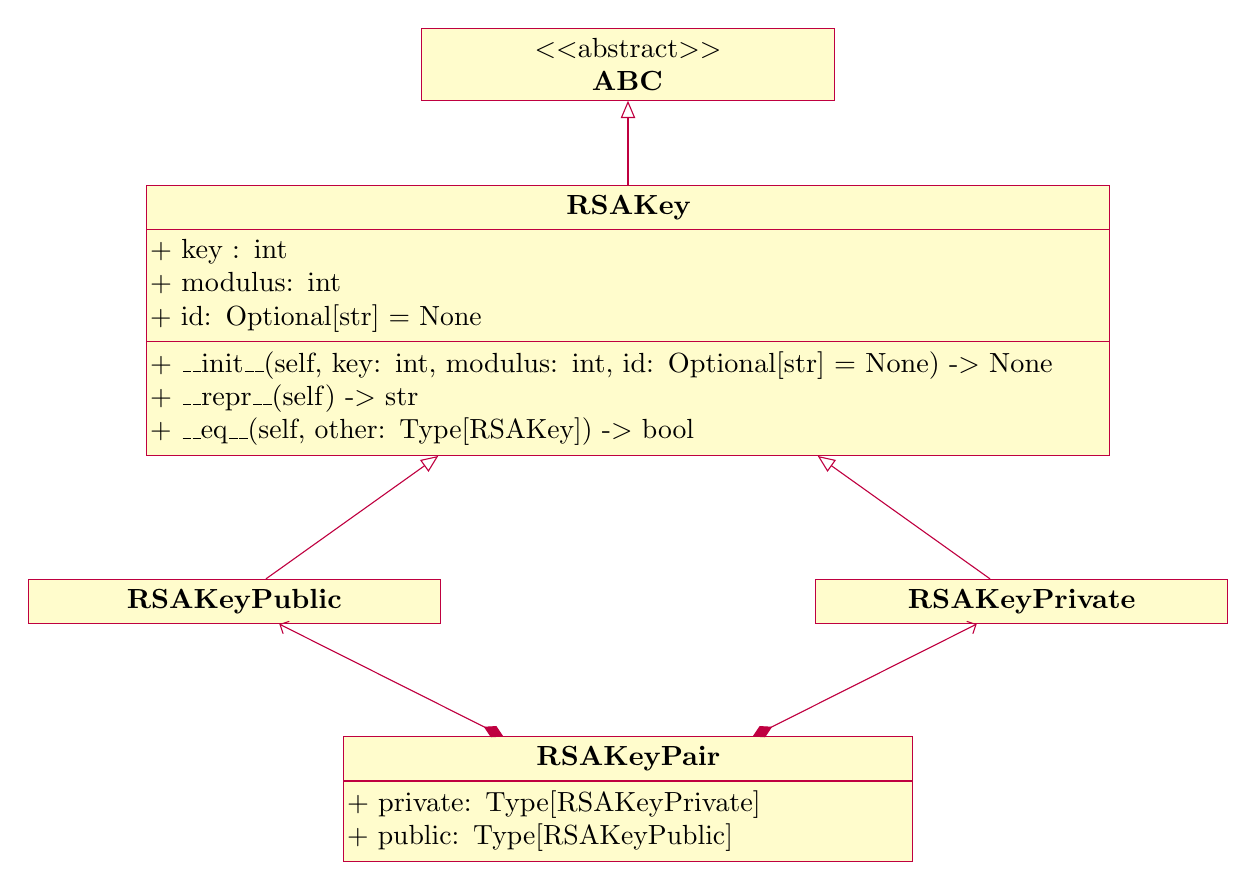
\begin{tikzpicture}
		\begin{abstractclass}[text width = 5 cm]{ABC}{0, 2}
		\end{abstractclass}
		\begin{class}[text width = 12 cm]{RSAKey}{0 ,0}
			\inherit{ABC}
			\attribute{+ key : int}
			\attribute{+ modulus: int}
			\attribute{+ id: Optional[str] = None}
			\operation{+ \textunderscore\textunderscore init\textunderscore\textunderscore(self, key: int, modulus: int, id: Optional[str] = None) -\textgreater\ None}
			\operation{+ \textunderscore\textunderscore repr\textunderscore\textunderscore(self) -\textgreater\ str}
			\operation{+ \textunderscore\textunderscore eq\textunderscore\textunderscore(self, other: Type[RSAKey]) -\textgreater\ bool}
		\end{class}
	
		
		\begin{class}[text width = 5 cm]{RSAKeyPublic}{ -5 , -5}
			\inherit{RSAKey}
		\end{class}
		\begin{class}[text width = 5 cm]{RSAKeyPrivate}{5 , -5}
			\inherit{RSAKey}
		\end{class}
	
	
		\begin{class}[text width = 7 cm]{RSAKeyPair}{0 , -7}
			\attribute{+ private: Type[RSAKeyPrivate]}
			\attribute{+ public: Type[RSAKeyPublic]}	
		\end{class}
	
	
		\composition{RSAKeyPair}{}{}{RSAKeyPrivate}
		\composition{RSAKeyPair}{}{}{RSAKeyPublic}
	\end{tikzpicture}
\end{document}